\documentclass[a4j,10pt,twocolumn]{utf8/abstract}
%\documentclass[a4j,9pt,twocolumn]{abstract}
\usepackage[dvipdfmx]{graphicx}
\usepackage[varg]{txfonts}
%%% \begin{document}の前に,各エントリーを記述する

\title{mruby Bytecode Loader Using Bluetooth in Multi-VM Environment}	% 論文のタイトル
\author{山本 拓朗} 		% 著者
\studentid{09C12174} 	% 学籍番号
\lab{潮}		% 研究室名

% 英語なら以下2行を定義
\englishtitle
\jptitle{Bluetoothを用いたマルチVM対応mrubyバイトコードローダ}  % 日本語のタイトル
 
\begin{document}
\absttitle 		% 表題の出力

\section{まえがき}
近年,組込みシステムは複雑化・大規模化しているため,組込みソフトウェアの生産性が問題になっている.

組込みソフトウェア開発の生産性の向上を目的として,mruby(軽量Ruby)を適用させたコンポーネントベース開発が可能なフレームワークであるmruby on TECSを提案してきた \cite{mrubyontecs}.

現状のmruby on TECSでは,プラットフォームにmrubyバイトコードを組み込んでいるため,mrubyプログラムを修正する度にコンパイル・リンクし直す必要がある.
さらに,マルチVMを提供しているが,複数のmrubyプログラムを効率よく並行動作させるには開発者がリアルタイムOSの機能を熟知している必要がある.

本研究では,mruby on TECSの拡張として,mrubyアプリケーションのバイトコードをBluetoothで転送することで開発効率を向上させる.
さらに,複数のmrubyプログラムを協調動作できるフレームワークを提案する.
\section{mruby on TECS}
mruby on TECSは,組み込み向けの高生産性なスクリプト言語のひとつであるmruby (軽量Ruby) と,組込みシステムに適したコンポーネントシステムであるTECS (TOPPERS Embedded Component System) を組み合わせた,組込みソフトウェアのコンポーネントベース開発が可能なフレーム―ワークである.

スクリプト言語は生産性が高い反面,C言語に比べると実行速度が遅いので,組込みシステムに適用するのは難しい.
mruby on TECSでは,mruby-TECS BridgeによってmrubyプログラムからC言語レベルの関数を呼ぶことが可能になっている.
mruby on TECSは,mrubyに比べて,アプリケーションを約100倍速く実行できる.

現状のmruby on TECSでは,mrubyアプリケーションを修正する度にホスト・ターゲットデバイス間でSDカードを抜き差し,再度OSを起動する必要がある.
その上,複数のmrubyアプリケーションを並列実行させる場合,開発者がタスクを待ち状態へ遷移させるようなOSの機能を呼び出さなければならない.
 
\section{提案フレームワーク}
提案フレームワークは,mruby on TECSをベースにしてBluetoothを用いたmrubyバイトコードローダと実用的なマルチタスク処理の実装を行った.
システムモデルを図\ref{fig:system_model}に示す.

\begin{figure}[h]
    \centering
    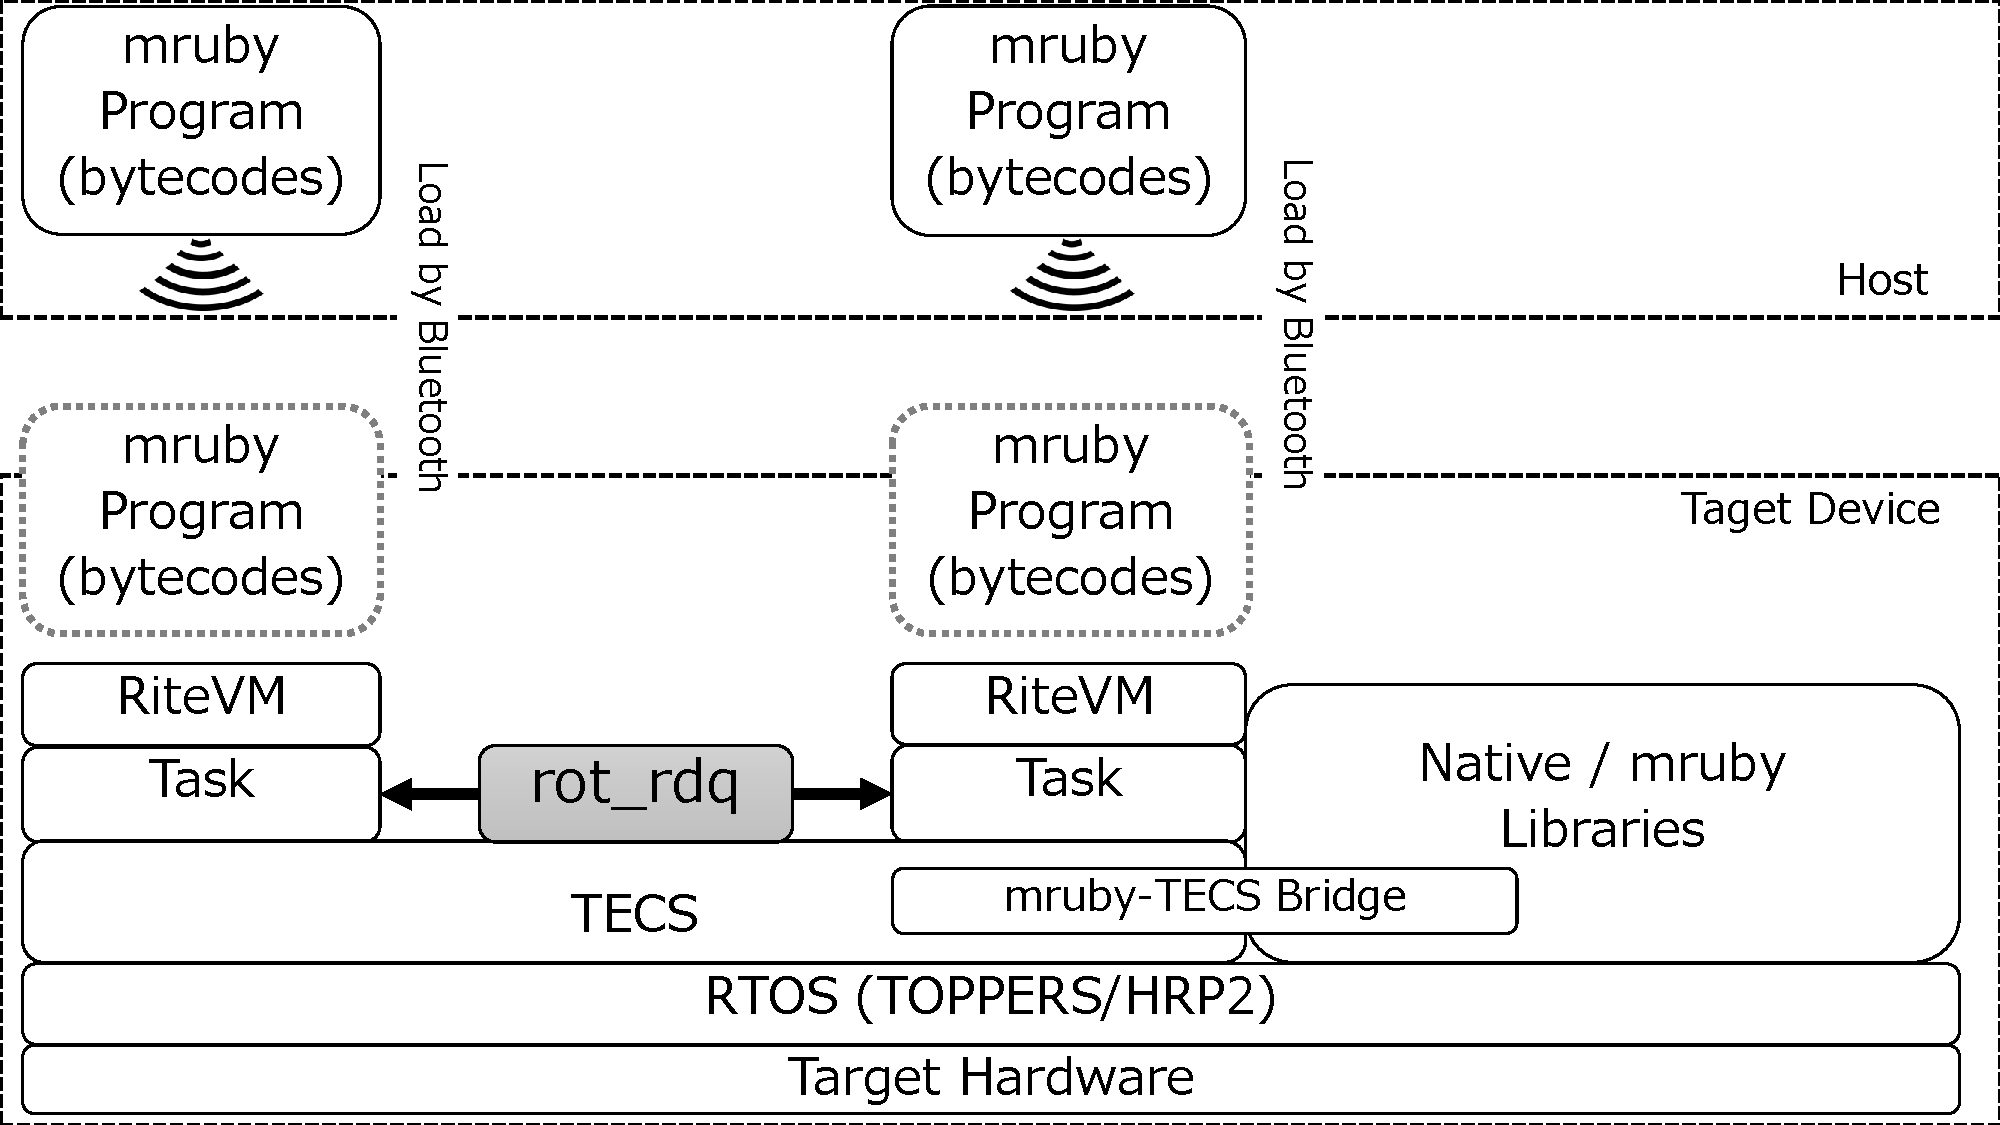
\includegraphics[width=8cm,clip]{figure/system_model.pdf}
    \caption{System Model}
    \label{fig:system_model}
\end{figure}

提案フレームワークでは,はじめの1度のみmrubyアプリケーション部分を除いたプラットフォームをコンパイル・リンクする.
ホスト側では,mrubyアプリケーション (.rb) をバイトコード (.mrb) にコンパイルし,Bluetoothを通してターゲットデバイスにバイトコードを送信する.
ターゲットデバイス側では,RiteVMに実装されたローダが送られたファイルを受信し,すでにリンクされているmrubyライブラリと合わせてアプリケーションを実行する.
この過程で開発することで,SDカードを抜き差しする手間やOSを起動し直す時間が省けるので,作業効率を上げることができる.

さらに,現状のmruby on TECSでは使用するのが難しかったマルチタスク処理を,$\mu$ITRON \cite{microITRON} のサービスコールである{\it rotateReadyQueue}を周期ハンドラで周期的に呼び出すことで,開発者にとって使いやすい設計にした.
{\it rotateReadyQueue}は,同じ優先度のタスクの実行順序を切り替える機能である.
複数タスク間の同期にはイベントフラグ処理を適用し,すべてのタスクが同時に起動するように実装した.
イベントフラグのセットパターンや待ちパターンは,各コンポーネントの属性として定義する.
これによって,VMの数に関わらず,同じ.cファイルを利用することが可能になる.

提案フレームワークでは,RiteVMや周期ハンドラ,イベントフラグはすべてTECSのコンポーネントとして実装されているので,開発者の必要に応じて機能を付けたり外したりすることも容易に実現できる.

\section{結論}
mruby on TECSの機能として,Bluetoothを用いたmrubyバイトコードローダと実用的なマルチタスク処理を提案した.
実験評価では,ローダによる作業効率の向上やオーバーヘッドの少ないマルチタスク設計の有用性を示した.


%\bibliographystyle{junsrt}
%\bibliography{refs}
\begin{thebibliography}{2}
\bibitem{mrubyontecs} Azumi, T. and Nagahara, Y. and Oyama, H. and Nishio, N., 
    ``mruby on TECS: Component-Based Framework for Running Script Program," 
    Proceedings of the 18th IEEE International Symposium on Real-Time Distributed Computing (ISORC), 
    pp.252-259, 
    2015. 

    \bibitem{microITRON} Hiroaki Takada and Ken Sakamura,
    ``$\mu$ITRON for Small-Scale Embedded Systems",
    IEEE Micro,
    vol.15,
    no.6,
    pp.46-54,
    1995.
\end{thebibliography}
\newpage
\pagebreak
\end{document}
